\documentclass[12pt,a4paper]{article}
\usepackage[utf8]{inputenc} %polskie znaki
\usepackage[T1]{fontenc}	%polskie znaki
\usepackage{amsmath}		%matematyczne znaczki :3
\usepackage{enumerate}		%Dodatkowe opcje do funkcji enumerate
\usepackage{geometry} 		%Ustawianie marginesow
\usepackage{graphicx}		%Grafika
\usepackage{wrapfig}		%Grafika obok textu
\usepackage{float}			%Allows H in fugire
\usepackage{hyperref}		%Allows hyperlinks
%\pagestyle{empty} 			%usuwa nr strony
\usepackage{todonotes}		%Todo notatki
\usepackage{lipsum}         %Lorem text
\usepackage{ntheorem}   	% for theorem-like environments
\usepackage{mdframed}   	% for framing
\usepackage{subcaption}		% subfigure (image placing)
\usepackage{pdfcomment}		% Komentarze (z bazowego pdf'a)
\usepackage{xparse}			% New commands with optional arguments
\usepackage{ifthen}			% If then - funkcje!
\usepackage{expl3}			% Deklarowanie zmiennych
\usepackage{pgf}			% Aktualne rachunki \pgfmathparse{}

\newgeometry{tmargin=2cm, bmargin=2cm, lmargin=2cm, rmargin=2cm} 

%Counter commands{
	\newcounter{counter} % Creates a new counter
	\setcounter{counter}{1} % Sets the counter to 5
	\newcommand{\counter}[1]{
		\arabic{#1} \stepcounter{#1} 
	}
	\newcommand{\counterreset}[1]{\setcounter{#1}{1}}
	%}

%Define styles{
	\theoremstyle{break}
	\theoreminframepreskip{0.5cm}
	\theoremheaderfont{\bfseries}
	\newmdtheoremenv[%
	linecolor=white,%
	innertopmargin=\topskip,
	shadowsize=0,%
	innertopmargin=5,%
	innerbottommargin=5,%
	leftmargin=10,%
	rightmargin=10,%
	backgroundcolor=gray!20,%
	innertopmargin=0pt,%
	ntheorem]{zad}{Zadanie}
	
	\mdfdefinestyle{zadanie}{
		linecolor=white,%
		innertopmargin=5,%
		innerbottommargin=5,%
		leftmargin=10,%
		rightmargin=10,%
		backgroundcolor=gray!20,%
		innertopmargin=8,
		innerbottommargin=8,
		skipabove = 5,
	}
	\mdfdefinestyle{wzor}{
		linecolor=cyan,%
		linewidth=2pt,%
		innertopmargin=8,
		innerbottommargin=8,
		leftmargin=10,%
		rightmargin=10,%
		backgroundcolor = white, 
		fontcolor = black,
		skipabove = 5,
		skipbelow = 5,
	}
	%}

%Zadania templatex%{
	\newcommand{\Wzor}[1]{
		\begin{mdframed}[style=wzor]
			\centering #1
		\end{mdframed}
	}
	\newcommand{\ZadanieTextowe}[1]{
		\begin{mdframed}[style=zadanie]
			\textbf{Zadanie \counter{counter} } \\
			#1
		\end{mdframed}
	}
	\newcommand{\Zadanie}[2]{
		\ZadanieTextowe{#1}
		#2
	}
	\newcommand{\ZadanieABCD}[6]{
		\ZadanieTextowe{#1}
		#2 \\\\
		\begin{tabular}{p{7cm} p{7cm}}
			\textbf{A. }#3&
			\textbf{B. }#4\\\\
			\textbf{C. }#5&
			\textbf{D. }#6\\
		\end{tabular}
	}
	\newcommand{\ZadanieABCDEF}[8]{
		\ZadanieTextowe{#1}
		#2 \\\\
		\begin{tabular}{p{7cm} p{7cm}}
			\textbf{A. }#3&
			\textbf{B. }#4\\\\
			\textbf{C. }#5&
			\textbf{D. }#6\\\\
			\textbf{E. }#7&
			\textbf{F. }#8\\\\
		\end{tabular}
	}
	\newcommand{\Zadanietwoxtwo}[5]{
		\ZadanieTextowe{#1}
		\begin{tabular}{p{7cm} p{7cm}}
			\textbf{a)} #2&
			\textbf{b)} #3\\\\
			\textbf{c)} #4&
			\textbf{d)} #5\\\\
		\end{tabular}
	}
	\newcommand{\Zadanietwoxthree}[7]{
		\ZadanieTextowe{#1}
		\begin{tabular}{p{7cm} p{7cm}}
			\textbf{a)} #2&
			\textbf{b)} #3\\\\
			\textbf{c)} #4&
			\textbf{d)} #5\\\\
			\textbf{e)} #6&
			\textbf{f)} #7\\\\
		\end{tabular}
	}
	\newcommand{\Zadanietwoxfour}[9]{
		\ZadanieTextowe{#1}
		\begin{tabular}{p{7cm} p{7cm}}
			\textbf{a)} #2&
			\textbf{b)} #3\\\\
			\textbf{c)} #4&
			\textbf{d)} #5\\\\
			\textbf{e)} #6&
			\textbf{f)} #7\\\\
			\textbf{g)} #8&
			\textbf{h)} #9\\\\
		\end{tabular}
	}
	\newcommand{\Informacja}[2]{
	\begin{mdframed}[style=zadanie]
		\textbf{Informacja do zadań \arabic{counter} - \pgfmathparse{\arabic{counter}+#1-1}\pgfmathprintnumber[assume math mode=true, int detect]{\pgfmathresult}}
	\end{mdframed}
	#2
	}
	
	%}

\newcommand{\tg}{\text{tg}}
\newcommand{\ctg}{\text{ctg}}
\newcommand{\UkladRownan}[2]{
	$\left\{
	\begin{array}{l}
		#1 \\
		#2
	\end{array}
	\right.$
}

\begin{document}
	\begin{center}
		\LARGE Funkcja wykładnicza i logarytmiczna
	\end{center}

	\Zadanietwoxfour{Oblicz stosując działania na potęgach:}
	{$4^5\cdot6^3:2^7=$}{$3^3:81^2\cdot 9^{10}=$}{$243^2:9^3=$}{$(33^3:11^3)^2:9^3=$}
	{$(18^2\cdot81^3)^2:(4\cdot3^{15})^2=$}{$(32^3)^5:64^5=$}{$12^5:3^{10}\cdot6^5=$}{\Large$\frac{4^3:8^2}{32:2^7}=$}
	
	\Zadanietwoxtwo{Oblicz:}
	{\Large$\frac{(1024-2^7)\cdot343}{2^7\cdot7^5}=$}
	{\Large$\frac{1080\cdot6^4+6^7}{(6^2)^3}=$}
	{\Large$\frac{8\cdot3^4\cdot3^{11}-9\cdot3^{12}}{46(3^{18}:3^4)}=$}
	{\Large$\frac{(5^{20}+5^{18}\cdot27^4)}{(5^{16}+5^{14})\cdot9^5}=$}
	
	\Zadanietwoxtwo{Oblicz stosując działania na potęgach}
	{$3^{-2}\cdot3^4=$}{$(4^{-5})^{-2}\cdot\frac{1}{2}^{-3}=$}
	{$2^{-8}:2^{-5}=$}{$\frac{2^{-3}:4^6\cdot32^{-3}}{64^7:16^{-3}}$}
	
	\Zadanietwoxthree{Uprość wyrażenie}
	{$4\sqrt{2}-3\sqrt{2}+8\sqrt{2}=$}{$\sqrt{18}+\sqrt{72}-\sqrt{162}=$}
	{$\sqrt{96}-\sqrt{14}\cdot\sqrt{21}=$}{$\sqrt{28}+\frac{1}{2}\sqrt{200}-4\sqrt{63}+\sqrt{242}=$}
	{\Large$\frac{4\sqrt{5}-\sqrt{72}+\sqrt{45}}{\sqrt{80}}=$}{\Large$\frac{\sqrt{24}-\sqrt{48}+\sqrt{216}}{\sqrt{12}}=$}
	
	\ZadanieTextowe{Udowodnij, że liczba 
	$$k=\frac{1}{1-\sqrt{2}}+\sqrt{2}$$
	jest liczbą całkowitą.}
	
	\Zadanietwoxthree{Zapisz w postaci $a^x$}
	{$\sqrt[3]{5}=$}{$\sqrt[3]{16}=$}
	{$\sqrt[3]{\sqrt{5}}=$}{$\sqrt{5\sqrt[3]{5}}=$}
	{$\sqrt[5]{3\sqrt{27}}=$}{$\sqrt[10]{10^4\sqrt[5]{10^{17}}}=$}
	
	\Zadanietwoxtwo{Oblicz}{$2\cdot0.5^{-1}+4\cdot8^\frac{2}{3}-27^{-1}\cdot3^4=$}
	{$\frac{1}{2}\cdot216^\frac{2}{3}+(21,37^3)^0-81^{0,64}\cdot9^{-3}=$}
	{$125^{\frac{4}{3}}\cdot0,2^{-7}:5^6-4^5:8^4\cdot128^2=$}{\Large$(\frac{3^{-13}+3^6-18^4}{2^7\cdot(\frac{1}{32})^{-3}:81^7})^0=$}
	\Wzor{$\log_ab=c \Leftrightarrow a^c=b$}
	\Wzor{$\log_ax+\log_ay=\log_ax\cdot y \qquad \log_ax-\log_ay=\log_a\frac{x}{y}$
	$$\log_ax^r=r\log_ax$$}
	\Wzor{$\log_aa^x=x \qquad\qquad\qquad \log_{a^y}a^x=\frac{x}{y}$}
	
	\Zadanietwoxfour{Oblicz:}
	{$\log_2128=$}{$\log_6216=$}
	{$\log_5\frac{1}{25}=$}{$\log_20,25=$}
	{$\log_33\sqrt{3}=$}{$\log_\frac{1}{2}\frac{1}{4\sqrt{2}}=$}
	{$\log_48=$}{$\log_\frac{1}{3}9\sqrt[4]{27}=$}
	
	\Zadanietwoxthree{Oblicz:}
	{$\log4+2\log_5=$}{$\log_218-\log_29=$}
	{$\log_50,2-\log_5\frac{1}{125}=$}{$\log_48+\log_432=$}
	{$\log_56,25+2\log_52=$}{$\log_\frac{1}{3}12\sqrt{3}+\log_\frac{1}{3}\frac{\sqrt{3}}{4}=$}
	
	\Zadanietwoxtwo{Naszkicuj wykres funkcji $f(x)=2^x$, a następnie na podstawie tego rysunku naszkicuj funkcję:}
	{$g(x)=2^{x-1}$}{$g(x)=2^{x}-5$}
	{$g(x)=2^{x-2}+4$}{$g(x)=\frac{1}{2}^x$}
	
	\ZadanieTextowe{Naszkicuj wykres funkcji $\log_2x$, a następnie wyznacz jej dziedzinę i zbiór własności.}
	
	\newpage
	\counterreset{counter}
	\begin{center}
		\LARGE Funkcja wykładnicza i logarytmiczna - zadania maturalne
	\end{center}

	\ZadanieABCD{Dane jest wyrażenie $\sqrt[4]{4\sqrt{16}}$. }{Wartość tego wyrażenia jest równa:}{2}{4}{$\sqrt[3]{4}$}{$\sqrt{2}$}
	
	\Informacja{3}{Poniżej przedstawiono fragment wykresu funkcji $f(x)=a^x$
		\begin{center}
			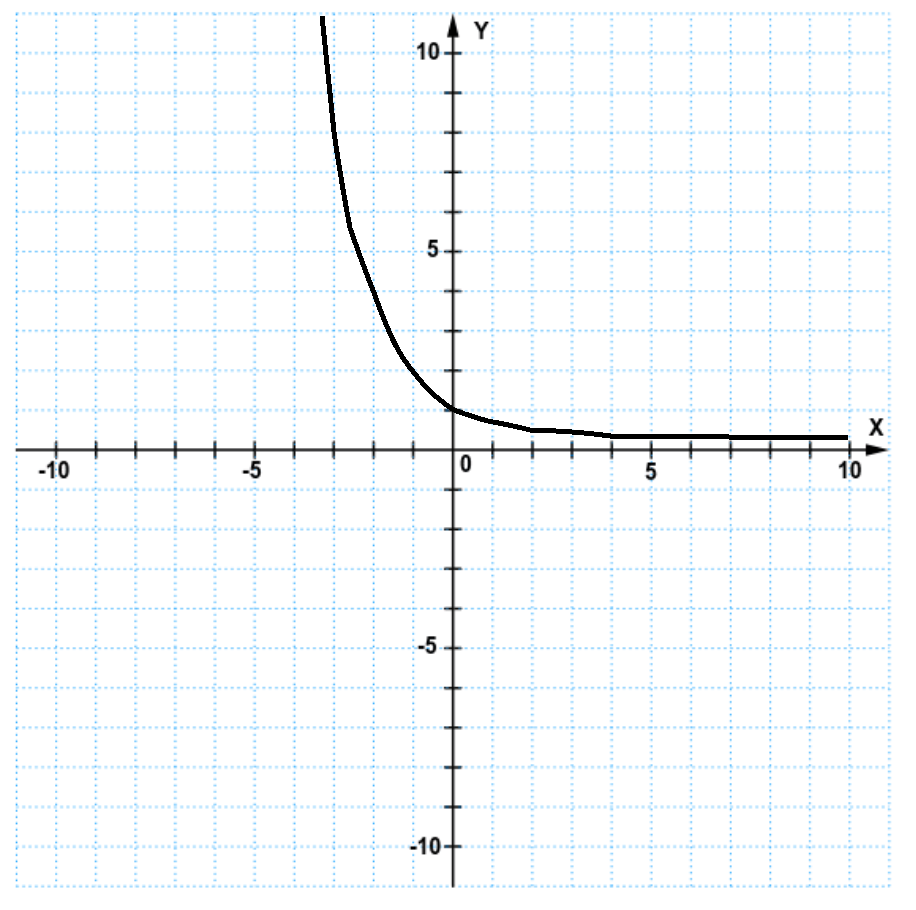
\includegraphics[scale=0.4]{6_1_1.png}
	\end{center}}
	
	\ZadanieABCD{Wartość tej funkcji dla argumentu -1 wynosi:}{\phantom{}}{$\frac{1}{2}$}{1}{0}{-$\frac{1}{2}$}
	\ZadanieTextowe{Wyznacz współczynnik "\textit{a}" dla tej funkcji.}
	\newpage
	\ZadanieABCD{Wyznacz który rysunek przedstawia wykres funkcji $g(x)=f(x-2)$}{\phantom{}}
	{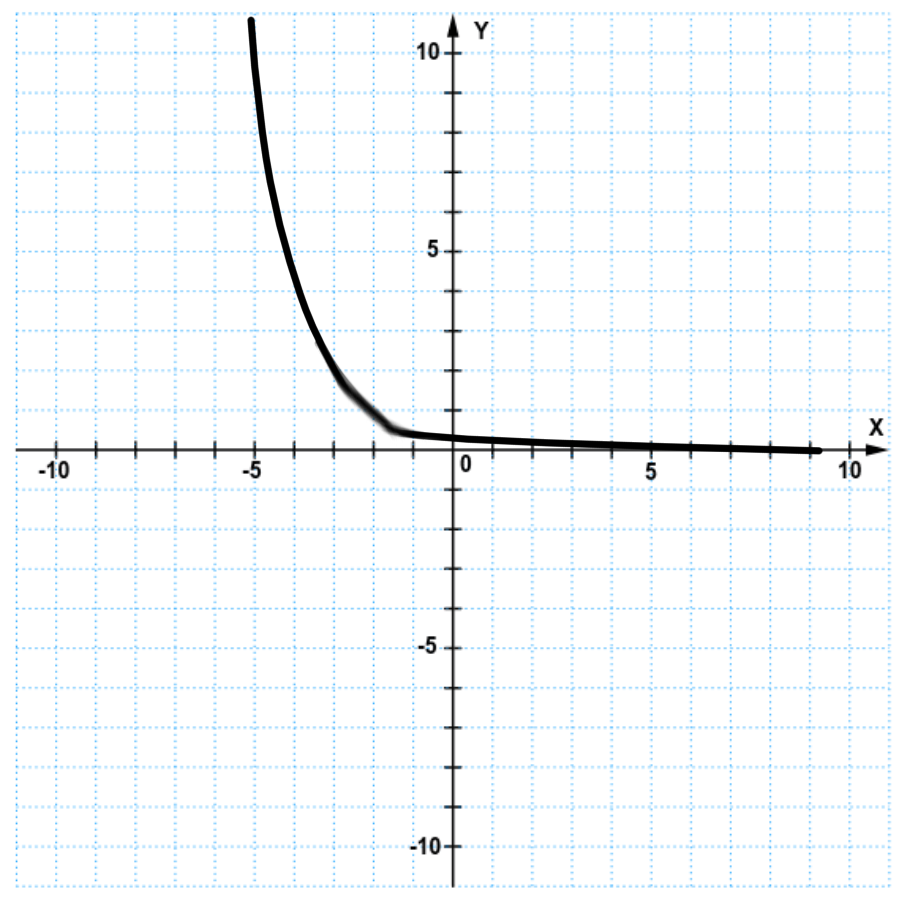
\includegraphics[scale=0.25]{6_1_2.png}}{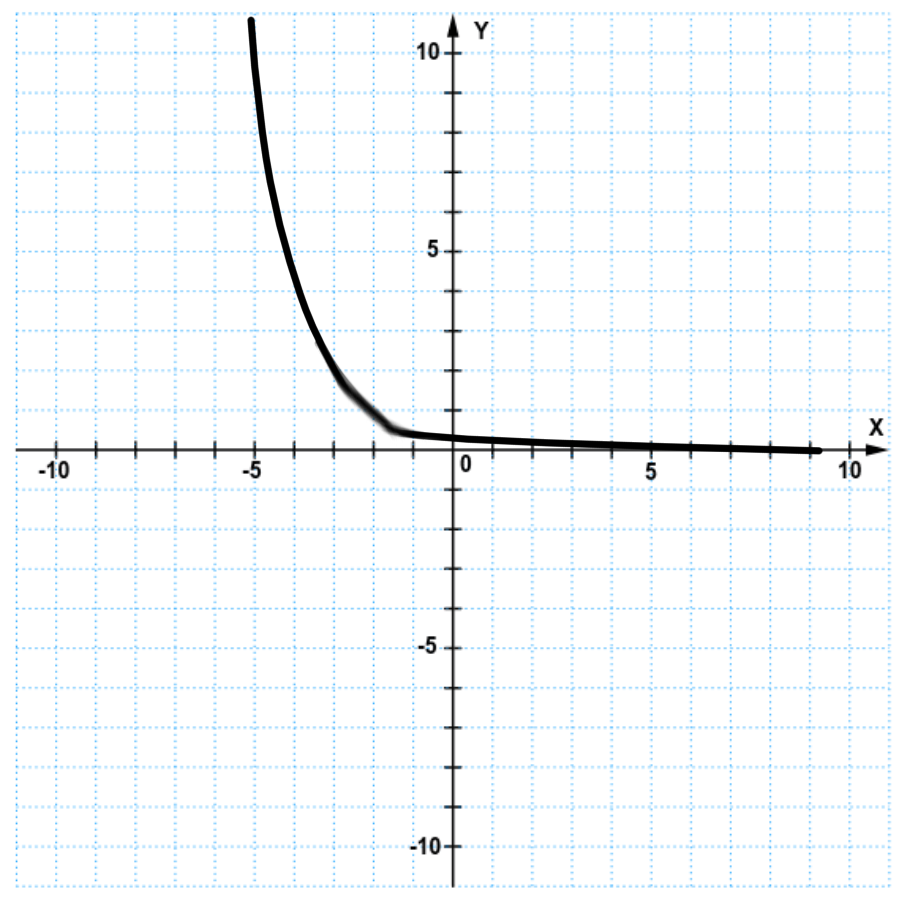
\includegraphics[scale=0.25]{6_1_2.png}}{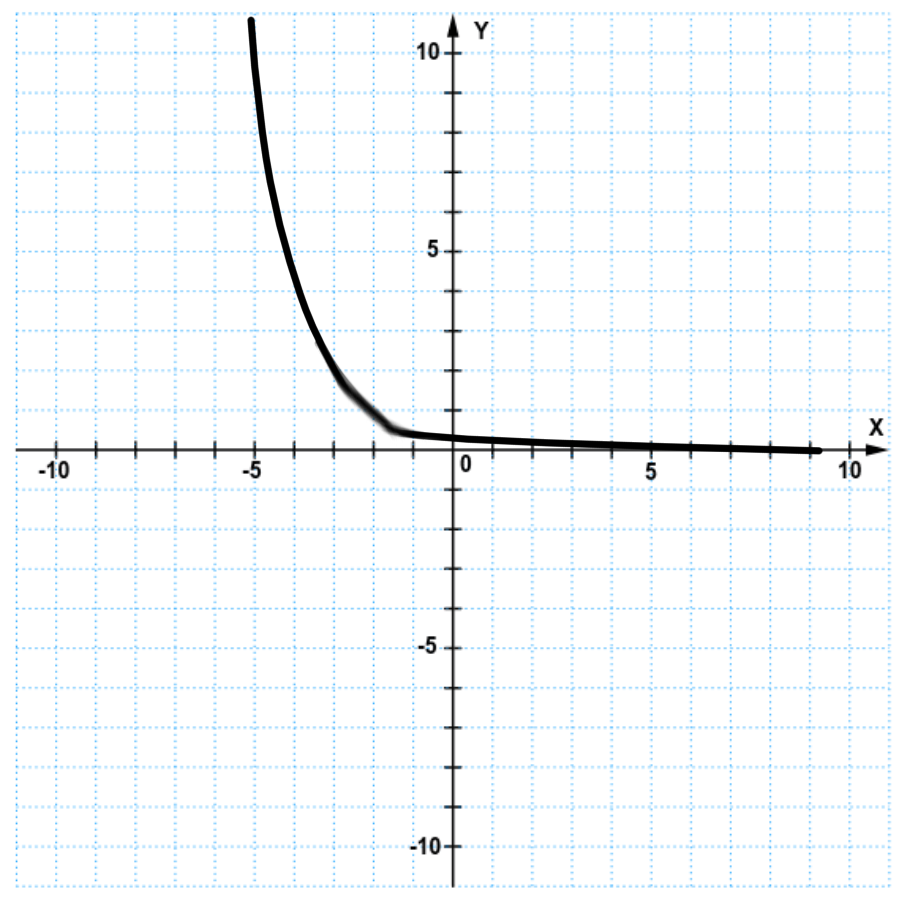
\includegraphics[scale=0.25]{6_1_2.png}}{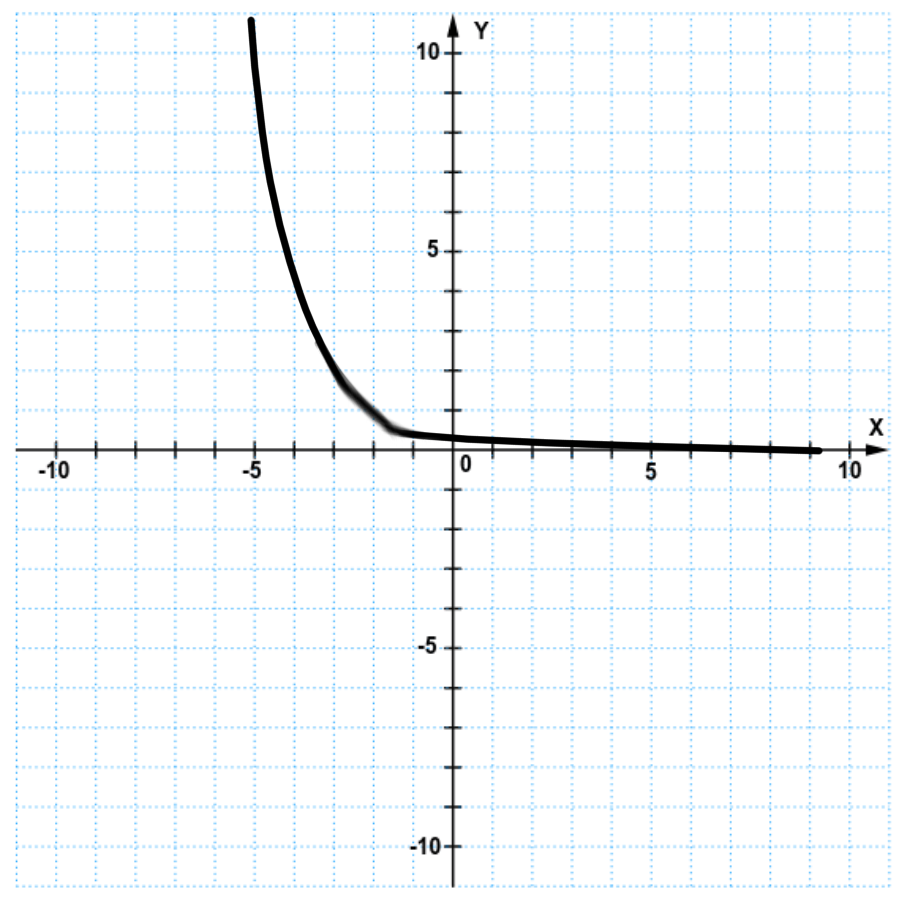
\includegraphics[scale=0.25]{6_1_2.png}}
	
	\ZadanieABCD{Dane jest wyrażenie $\log_654-2log_618$.}
	{Wartość tego wyrażenia da się zapisać jako}{-1}{$\log_618$}{$\frac{3}{2}$}{-2}

\end{document}